\chapter{Assurance Cases and Selected Evidence for AortaGeomRecon}

This chapter discusses building the evidence to support each claim of our AC  for AGR (AortaGeomRecon). We start from the top level claims of the AC developed in previous work \cite{scs_ac} and drill down to find the evidence that can support the arguments and the top level claims. The following material is presented in this chapter as part of the evidence: the Software Requirements Specification (SRS) of AGR, the Design Document, the Module Guide, the Test Plan, the Algorithm Review,  the User Manual, the User Instruction Video, AGR's control sequence, and a Warning Message implemented in AGR.

\section{Assurance Case Development}

Assurance Cases are build with claims, subclaims, contexts and evidence. The parts of  the AC  add up  to an argument that justifies that top level claim. By using \href{https://astah.net/products/astah-system-safety/}{Astah System Safety} software to present the Goal Structuring Notation (GSN) arguments \cite{Astah_2023}\cite{kelly2004goal}, we show that our software delivers correct outputs when used for its intended use/purpose in its intended environment, and within its assumed operating assumptions. Figure~\ref{fig_agr_ac_top} shows the top level of the assurance cases. With the goal of arguing that the software delivers correct outputs, we decompose the goal into four sub goals: GR, GI, GA and GBA, where GR stands for the goal of correct requirements of the software, GI stands for the goal of the implementation  matching the requirements, GBA is the goal of  that all  operational assumptions have been defined, and GA is the goal that all operational assumptions are met.

\begin{figure}[hp]
    \centering
    \fbox{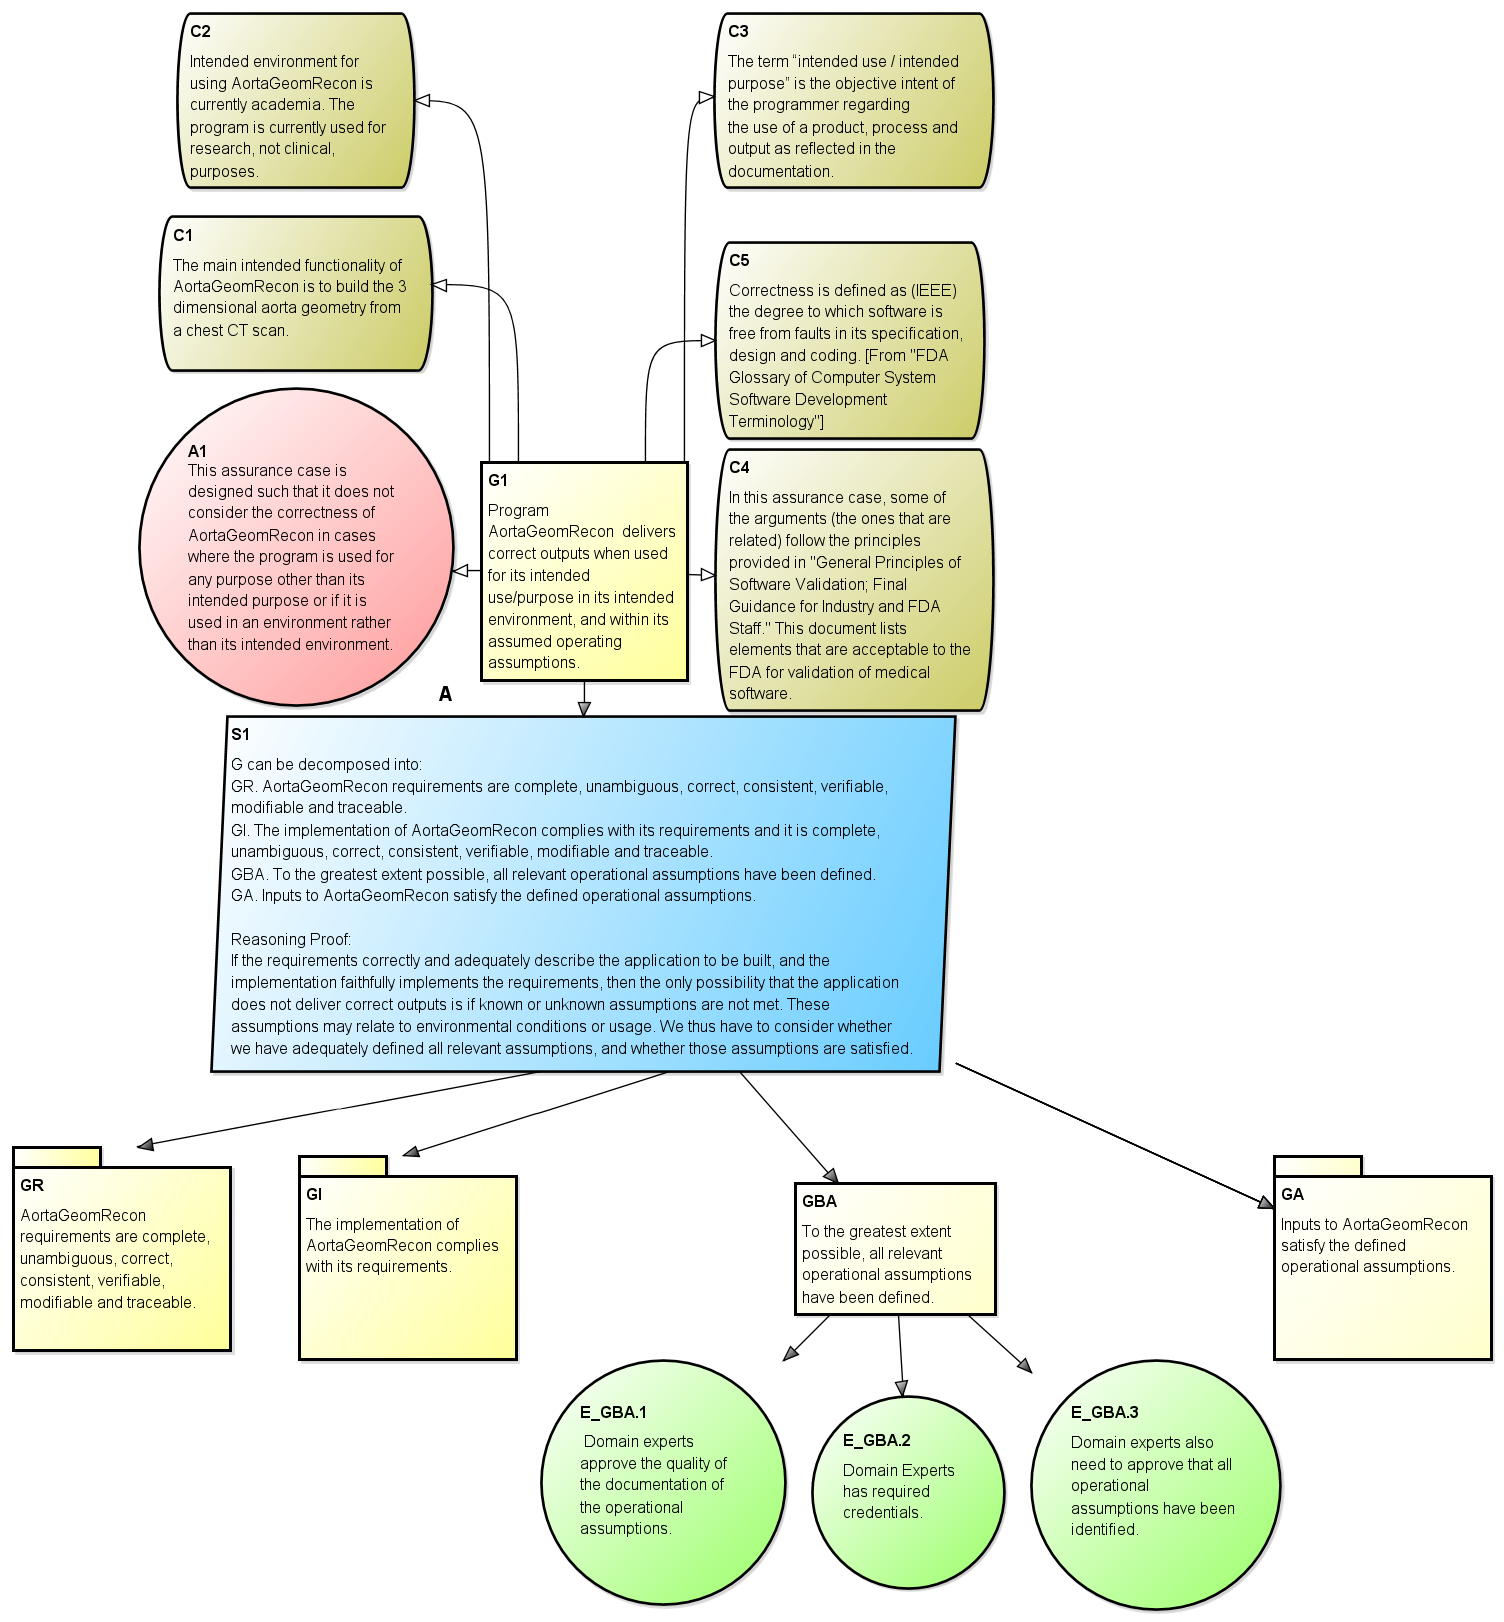
\includegraphics[width=0.99\textwidth]{figures/AC/Top_Level.png}}
    \caption[AGR Assurance Cases Top Level]{AGR Assurance Cases Top Level}
    \label{fig_agr_ac_top}
\end{figure}


\section{Assurance Case for Software Specification Requirements}

The first goal for getting trusted software is having a complete, unambiguous, correct, consistent, verifiable, modifiable and traceable SRS that shows the complete breakdown of the requirements with mathematical notation, data models and instance models. The SRS is the foundation of the software development, as the design and the implementation are created to satisfy the requirements document.

Figure~\ref{fig_agr_ac_gr} demonstrates the claims on the goal of correct requirements for AGR. On the left branch, GR\_3C states the goal of complete, correct, and consistent documentation. Under this claim, the goal is separated based on each characteristic, and the corresponding evidence is presented as the leaf nodes.

\begin{figure}[hp]
    \centering
    \fbox{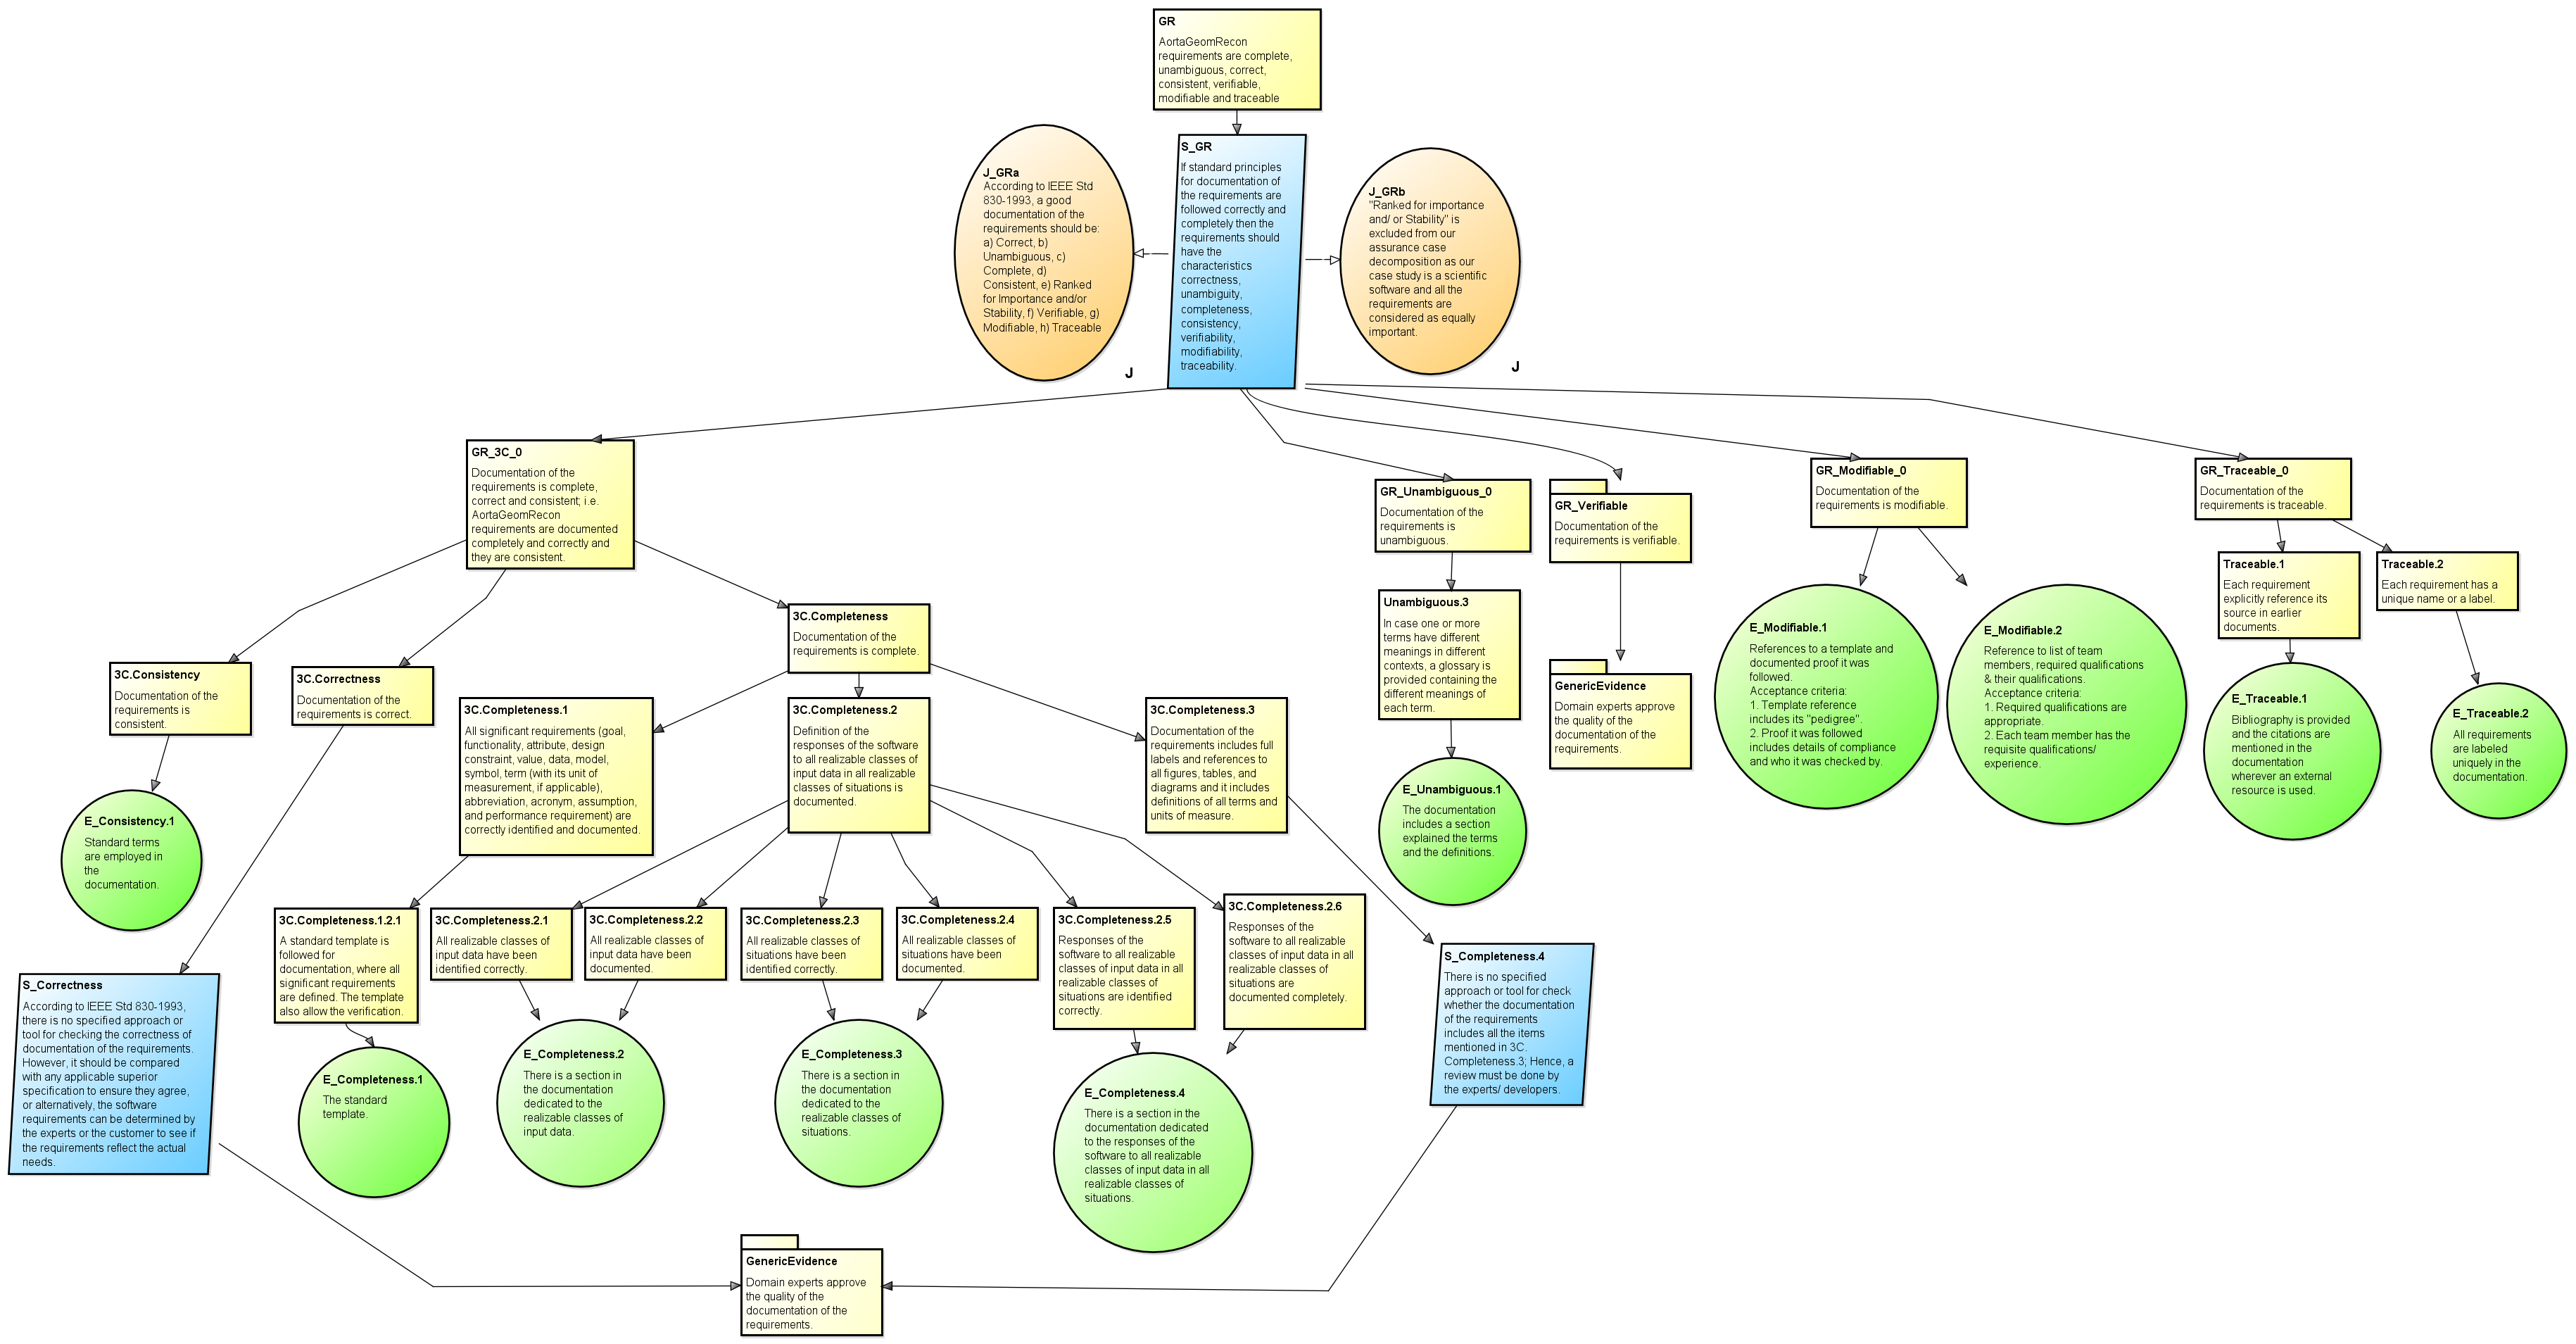
\includegraphics[width=1.3\linewidth, angle=90]{figures/AC/SRS/GSN_GR.png}}
    \caption[AGR Assurance Cases GR]{AGR Assurance Cases GR}
    \label{fig_agr_ac_gr}
\end{figure}

As shown in the assurance case GR, one of most important pieces of evidence for the SRS having these characteristics is that it follows a standard template. Using  a standard template builds confidence that all necessary requirements have been defined. Moreover, standardization allows a domain expert who has used this template to verify the quality of the document. The current work uses a template tailored for research software \cite{Smith2006}, which is the standard template in the evidence E\_Completeness.1 (Figure~\ref{fig_agr_ac_gr}), and all other evidences where a template is included.

\subsection{The sections of the SRS}
The full SRS for AGR is reproduced in Appendix \ref{SRS}. Excerpts from the SRS are used in the body of this report to show the document and illustrate the evidence it provides for the AC.
The table of content of the SRS is provided in Figure~\ref{fig_agr_srs_toc}. Some of the most important sections are explained below.
\begin{figure}[hp]
\fbox{\parbox{\textwidth}{
 \begin{myEnumerate}
	\item Reference Material
	\begin{myEnumerate}
	\item Table of Units
	\item Table of Notations
	\item Table of Symbols
	\item Abbreviations and Acronyms
	\end{myEnumerate}
	\item Introduction
	\begin{myEnumerate}
	\item Purpose of Document
	\item Scope of Requirements
	\item Organization of Document
	\end{myEnumerate}
	\item General System Description
	\begin{myEnumerate}
	\item System Context
	\item User Characteristics
	\item System Constraints
	\end{myEnumerate}
	\item Specific System Description
	\begin{myEnumerate}
	\item Problem Description
	\begin{myEnumerate}
	\item Background
	\item Terminology Definition
	\item Coordinate Systems
	\item Physical System Description
	\item Goal Statements
	\end{myEnumerate}
	\item Solution Characteristics Specification
	\begin{myEnumerate}
	\item Assumptions
	\item Theoretical Models
	\item Data Definitions
	\item Instance Models
	\item Data Constraints
	\item Properties of a Correct Solution
	\end{myEnumerate}
	\end{myEnumerate}
	\item Requirements
	\begin{myEnumerate}
	\item Functional Requirements
	\item Non-functional Requirements
	\end{myEnumerate}
	\item Other System Issues
	\item Traceability Matrix
	\item Likely Changes
    \end{myEnumerate}
}}
    \caption[AGR SRS Table Of Content]{AGR SRS Table Of Content}
    \label{fig_agr_srs_toc}
\end{figure}

\begin{itemize}
\item Reference Material

In this section, a Table of Symbols and an abbreviations and acronyms table are used to explain every symbol and Abbreviations used in the document. These tables ensure the consistency and the unambiguous characteristics of the document, providing evidence for E\_Consistency.1 and E\_Unambiguous.1 shown in Figure~\ref{fig_agr_ac_gr}. They are located at the very beginning of the document, so that the reader can first look at these tables before reading the entire document. 

\item Introduction

The introduction section defines the problem and the scope of the document.  There are subsections for explaining the purpose of document, abstracting the scope of the requirements and defining the characteristics of the intended reader. This section is provided for the reader to reduce the chance of an unqualified reader finding the document ambiguous.

\item General System Description

The general system description includes a system context diagram that explains the relationship between the users, the inputs given by the user and the outputs of the AGR program. Along with the figure, user responsibilities and AGR responsibilities are also defined in this section.

\item Specific System Description

This section presents more detail about the problem and the specific system to solve the problem. The first subsection, Problem Description, discusses the definition of Organ Segmentation, the Coordinate Systems used in medical image problems, and the Goal Statements. The goal for AGR is to extract the three-dimensional segmentation of the aorta.

\hspace{\enumerateparindent}The next subsection, Solution Characteristics Specification, starts with the assumptions, as shown in Figure~\ref{fig_agr_srs_a},  to clearly define the scope of the requirements. The subsection Data Definitions, defines Voxel, Image/Slice, and Volume with mathematical notation so that the developer can interpret unambiguously the definitions, as shown in Figure~\ref{fig_agr_dd}.  The Data Definitions subsection provides evidence for E\_Unambiguous.1 (Figure~\ref{fig_agr_ac_gr}).

\hspace{\enumerateparindent}Finally, the subsection Instance Models, shows the mathematical meaning of Region of Interest, as reproduced in Figure~\ref{fig_agr_im1}, and Segmentation in Figure~\ref{fig_agr_im2}. These are two essential models that the developer must know for developing their solution. The Assumptions, Data Definitions, and Instance Model sections provide evidence for E\_Completeness.2, E\_Completeness.3 and E\_Completeness.4, which states that there is a section in the documentation dedicated to the realizable classes of input data, realizable classes of situation and the response of the software to all realizable classes of input data in all realizable classes of situation. The Assumptions and the Data Definition sections define the realizable classes of input data. The Instance Model section defines the realizable classes of situation and the response of the software.

\begin{figure}[H]
    \centering
    \fbox{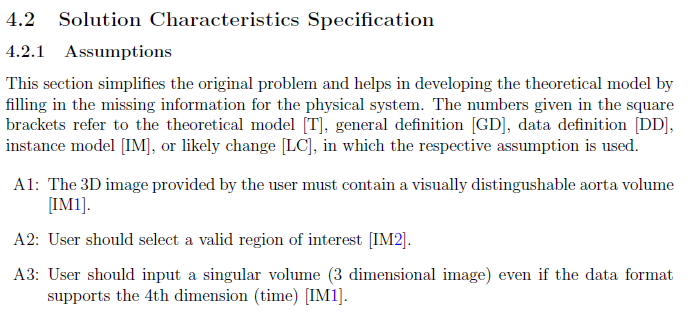
\includegraphics[width=\textwidth]{figures/AC/SRS/Assumptions.png}}
    \caption[AGR SRS Assumptions]{AGR SRS Assumptions}
    \label{fig_agr_srs_a}
\end{figure}

\begin{figure}[H]
    \centering
    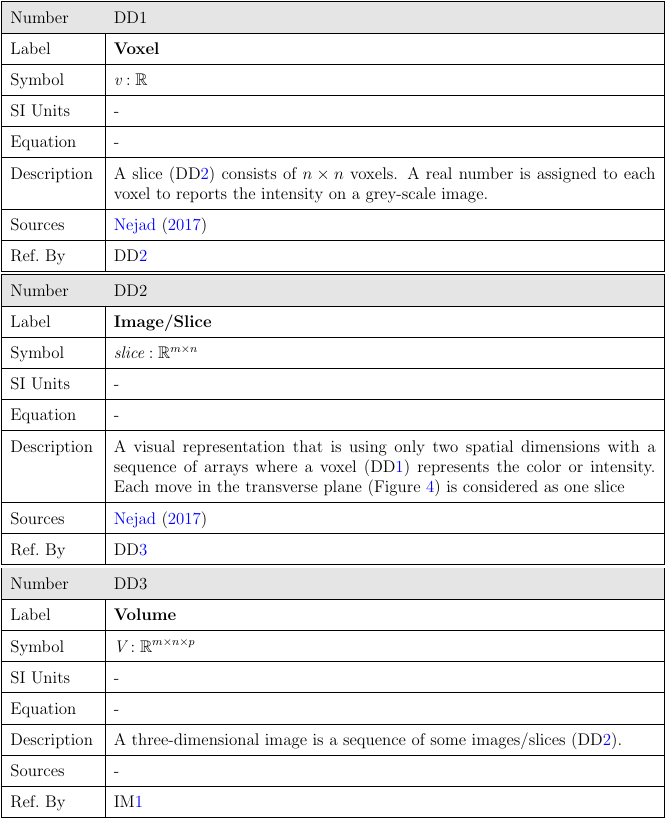
\includegraphics[width=\textwidth]{figures/AC/SRS/DD.png}
    \caption[AGR SRS Data Definitions]{AGR SRS Data Definitions}
    \label{fig_agr_dd}
\end{figure}

\begin{figure}[H]
    \centering
    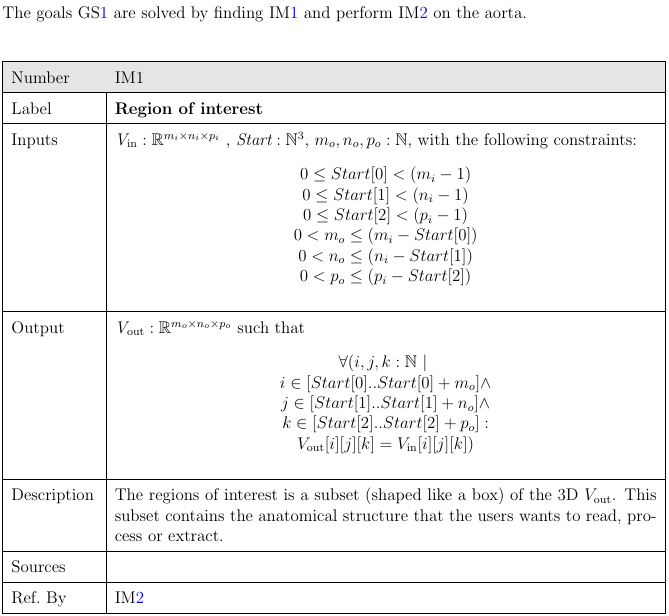
\includegraphics[width=\textwidth]{figures/AC/SRS/im1.png}
    \caption[AGR SRS Instance Model Region Of Interest]{AGR SRS Instance Model Region Of Interest}
    \label{fig_agr_im1}
\end{figure}

\begin{figure}[H]
    \centering
    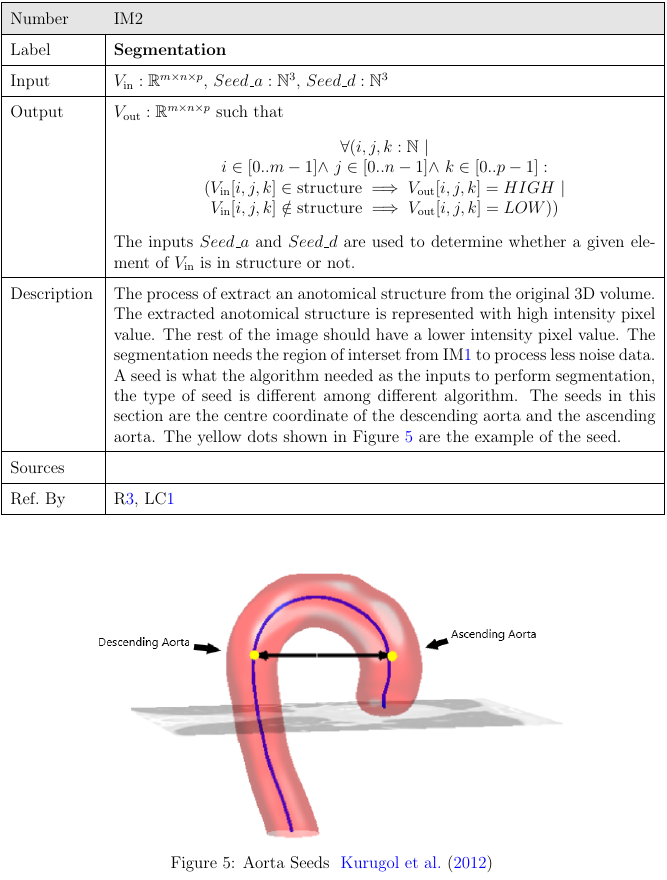
\includegraphics[width=\textwidth]{figures/AC/SRS/im2.png}
    \caption[AGR SRS Instance Model Region Of Interest]{AGR SRS Instance Model Region Of Interest}
    \label{fig_agr_im2}
\end{figure}


\item Requirements

With all the background information provided, the Functional Requirements and the Non-Functional Requirements can be presented for AGR. The Functional Requirements are defined by using the terms given in the Data Definitions, Instance Model, and based on the other Functional Requirements, as shown in Figure~\ref{fig_agr_fr}. To be verifiable, the Non-Functional Requirements usually have a measurement such as execution time, or the amount of manual effort. Figure~\ref{fig_agr_nfr} demonstrates the Non-Functional Requirements of Usability, Safety, Learnability, Accuracy and Consistency. The Functional Requirements and Non-Functional Requirements are labeled, which provides the evidence  for E\_Traceable.2 (Figure~\ref{fig_agr_ac_gr}).


\begin{figure}[H]
    \centering
    \fbox{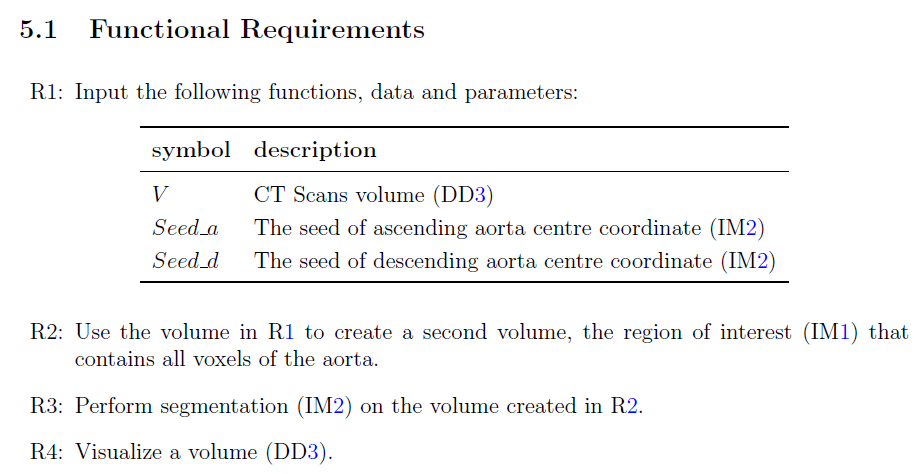
\includegraphics[width=\textwidth]{figures/AC/SRS/Functional_Requirements.png}}
    \caption[AGR Functional Requirements]{AGR Functional Requirements}
    \label{fig_agr_fr}
\end{figure}

\begin{figure}[H]
    \centering
    \fbox{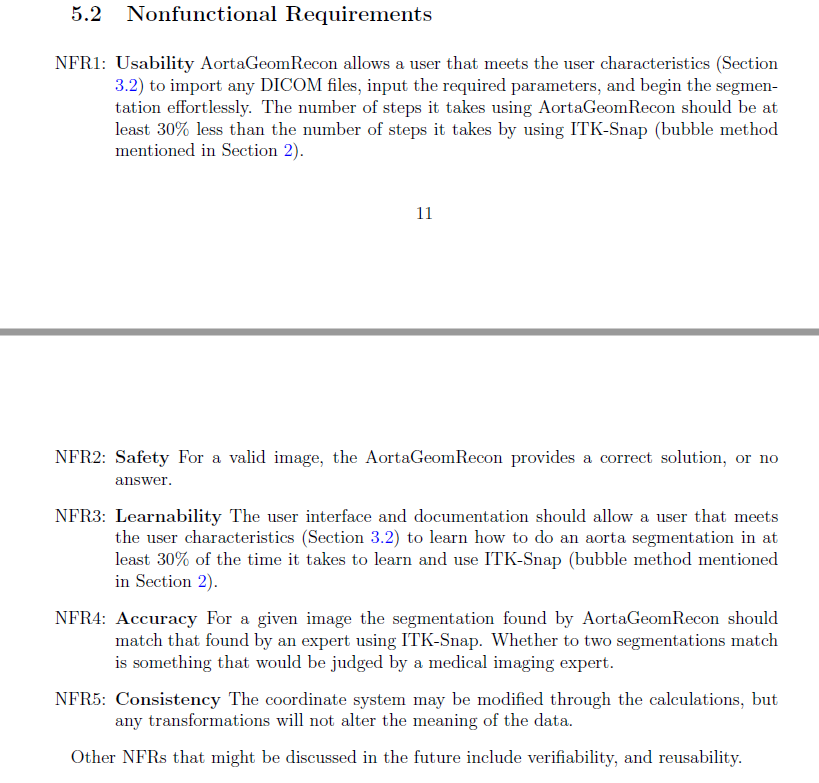
\includegraphics[width=0.75\textwidth]{figures/AC/SRS/NonFunctional_Requirements.png}}
    \caption[AGR Non- Functional Requirements]{AGR Non- Functional Requirements}
    \label{fig_agr_nfr}
\end{figure}

\item Likely Changes and Unlikely Changes

This section discusses the likely changes that the developer might expect in the future, and the unlikely changes along with their justification. The only likely change discussed in the AGR's SRS is regarding the segmentation method. For different segmentation methods, the inputs varies, since the segmentation method is a likely change, the inputs variables are also likely changes. The only unlikely change documented is the method of retrieving a region of interest. Currently, the standard approach is used of taking a starting point and sizes in different dimensions to get the region of interest.

\item Traceability Matrix and Graphs

The traceability matrices provide easy references on what has to be modified if a certain component is changed. Figure~\ref{fig_agr_tm_dd_im} is the traceability matrix of the Data Definitions and Instance Models. Figure~\ref{fig_agr_tm_im_r} shows the relationship between the requirements and other sections, and Figure~\ref{fig_agr_tm_a} shows the relationship between the assumptions and other sections.
\begin{figure}[H]
    \centering
    \fbox{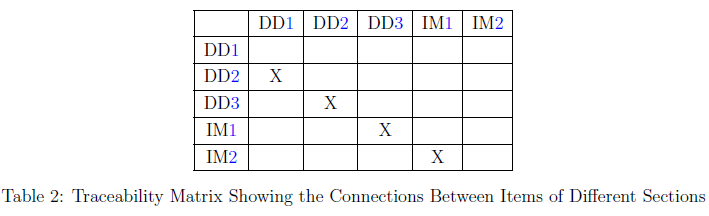
\includegraphics[width=0.7\textwidth]{figures/AC/SRS/tm_dd_im.png}}
    \caption[AGR Traceability Matrix between Data Definitions and Instance Model]{AGR Traceability Matrix between Data Definitions and Instance Model}
    \label{fig_agr_tm_dd_im}
\end{figure}

\begin{figure}[H]
    \centering
    \fbox{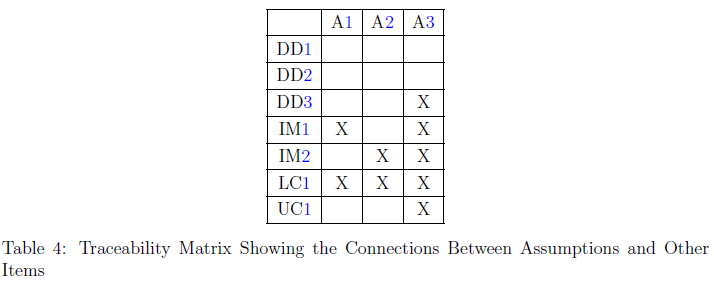
\includegraphics[width=0.8\textwidth]{figures/AC/SRS/tm_a.png}}
    \caption[AGR Traceability Matrix Between Assumptions and Other sections]{AGR Traceability Matrix Between Assumptions and Other sections}
    \label{fig_agr_tm_a}
\end{figure}

\begin{figure}[H]
    \centering
    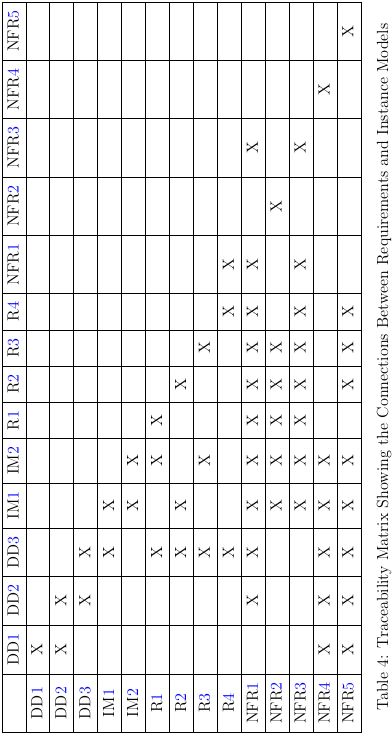
\includegraphics[width=0.7\textwidth]{figures/AC/SRS/tm_im_r.png}
    \caption[AGR Traceability Matrix Between Requirements and Other sections]{AGR Traceability Matrix Between Requirements and Other sections}
    \label{fig_agr_tm_im_r}
\end{figure}



\item Bibliography

A bibliography is provided at the end of SRS, the bibliography points to the template \cite{Smith2006} used for this documentation, and a list of citations for the external resources. This information is related to the evidence for E\_Traceable.1, which states that a bibliography is provided to include the citations of the external resource. The template is also related to E\_Modifiable.1, which states that the documentation references a template and provides proof it was followed.

\end{itemize}

\subsection{Documentation Review}

Documentation review is necessary to ensure that documentation is correct and complete. For the current project,  when there is an update in the documentation, GitHub issues were used to post a documentation review request, as shown in Figure~\ref{fig_agr_doc_review}. All documents and changes were reviewed by Dr. Spencer Smith, who has the requisite qualifications/experience to review the completeness and the correctness of the documentation. Additionally, the goal of the requirements being verifiable is also reviewed by Dr. Spencer Smith. For example, he reviewed the mathematical expression and helped define the terms in Data Definitions and Instance Model correctly and unambiguously. Therefore, the documentation review provides evidence for S\_Verifiable.

\begin{figure}[H]
    \centering
    \fbox{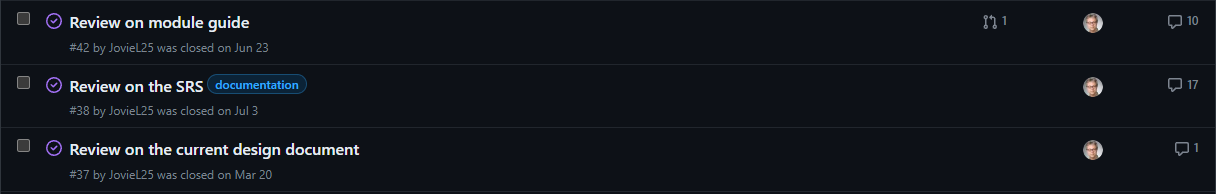
\includegraphics[width=\textwidth]{figures/AC/SRS/Git_issues.png}}
    \caption[GitHub Repo Documentation Review Requests]{GitHub Repo Documentation Review Requests}
    \label{fig_agr_doc_review}
\end{figure}


\section{Assurance Case for the Implementation}
The goal of implementation is that it fully complies with the SRS. As Figure~\ref{fig_agr_ac_gi} shows, we argue this in two ways:

\begin{enumerate}
  \item We argue that the implementation of the requirements has been verified.
  \item We argue the design matches the requirement and that the implementation complies with the design, which together implies that the implementation matches the requirements.
\end{enumerate}

\begin{figure}[hp]
    \centering
    \fbox{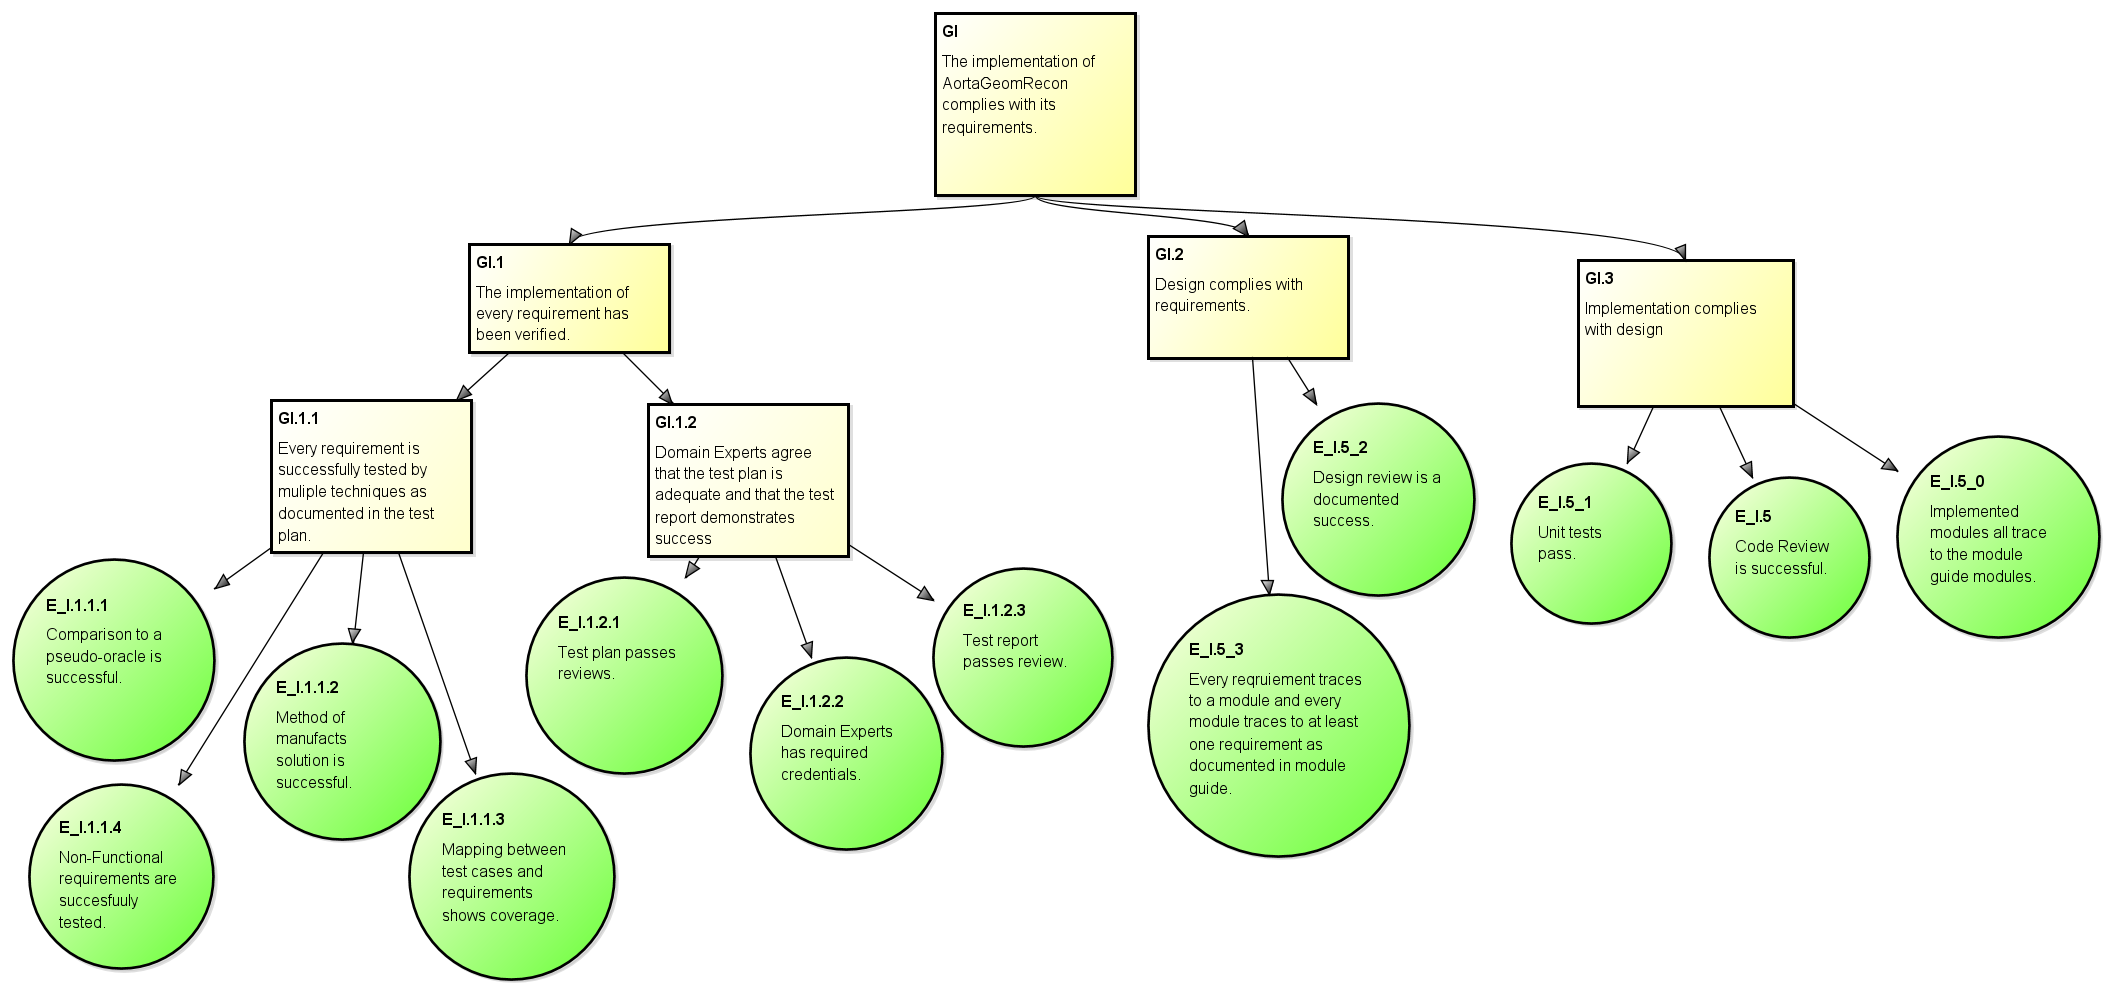
\includegraphics[width=1.3\linewidth, angle=90]{figures/AC/GI/GSN_GI.png}}
    \caption[AGR Assurance Cases For Implementation]{AGR Assurance Cases For Implementation}
    \label{fig_agr_ac_gi}
\end{figure}

This section focuses on matching the developed artifacts to the evidence shown in Figure~\ref{fig_agr_ac_gi}. The first subsection discusses the test plan of the AGR, particularly the continuous integration test infrastructure, test cases and the test procedure for testing all requirements of the software. Next, this section shows the design documents, including the Module Guide, which documents system architecture, and a design document for a detailed design explanation. Finally, we present the Code Walkthrough and the Algorithm Review, which helped us to eliminates bugs, errors, and increase our confidence in the implementation's completeness, and correctness.

\subsection{Test Plan}

GI.1 states the goal of the implementation of every requirement has been verified, so we need a test plan that is approved by a Domain Expert who has the required credentials,  and the tests cases cover all the Functional Requirement and Non-Functional Requirements. Unlike ITK-Snap's bubble method and 3D Slicer's threshold segmentation method that can interactively control the wanted pixels, our algorithm functions like a black box. With a given set of inputs and hyperparameters, we can only verify the result after the segmentation.

This section discusses on how ``Ground Truth'' was built with a verified version of the algorithm, and then compared it using Dice Similarity. Next, GitHub Actions are shown for managing the workflows, for the continuous integration infrastructure that performs static code analysis and continuous integration tests. Then, a test procedure to cover the Functional Requirements and Non-Functional Requirements is provided, as the evidences for GI.1 in Figure~\ref{fig_agr_ac_gi}. Finally, the test plan approval and the test report are discussed as artifacts related to the evidences for GI.1.2.

\subsubsection{Build ``Ground Truth'' Data}
For the current project, we did not have the time and resource to manually build our ``Ground Truth'' test cases using ITK-Snap; therefore, we built the ``Ground Truth'' test cases using the previously verified version of the algorithm (written by Kailin) with a set of tuned hyperparameters. The process of building the test case data is described as follows:

\begin{enumerate}
  \item Generate test case data with the previous version of the algorithm.
  \item Generate test case data with the new version of the algorithm.
  \item Calculate the Dice Similarity Coefficient (DSC) of the two test case data.
  \item Determine whether there is a strong difference in the DSC value, and use a visualization tool, such as 3D Slicer, to see the actual difference. As long as the difference is small, the test case is assumed to pass.
\end{enumerate}

The Dice Similarity Coefficient (DSC) was used as a statistical validation metric to evaluate the performance of both the reproducibility of manual segmentations and the spatial overlap accuracy of automated probabilistic fractional segmentation of MR images \cite{ZOU2004178}. The equation of DSC with boolean data, using the definition of true positive (TP), false positive (FP), and false negative (FN), is written as \cite{Wikipedia_2023}:
\begin{equation}
DSC = \frac{2TP}{2TP+FP+FN}
\end{equation}
The value of a DSC ranges from 0, indicating no spatial overlap between two sets of binary segmentation results, to 1, indicating complete overlap \cite{ZOU2004178}. With a large DSC value (0.95), the evidence E\_1.1.1 is achieved by comparing a new generated result with a pseudo-oracle. The statement of the evidence E\_1.1.2 is also correct, which implies that a chosen approach or methodology has led to the creation of software that functions as intended, meets user requirements, and adheres to quality standards.

\subsubsection{GitHub Actions workflows}\label{ci}
Our Continuous Integration infrastructure was implemented with a GitHub Actions workflow. A workflow is a configurable and automated process that will run one or more jobs on the software projects when there is a commit or a pull request. GitHub Actions uses a YAML file to define the events and the commands to be executed on its temporary container \cite{GitHubActions}.

For AGR there are two automated process that happens on each ``push" event and ``pull" event. A ``push" event implies that something is changed in one or multiple commits, therefore there is a need to verify whether the commits have introduced bugs. A ``pull" event happens when a feature branch is merged with the main branch. Since our main branch is protected, any update to the main branch must be merged by using a pull-request. Before a pull-request can be approved, the continuous integration tests are examined. 

The first automated process is a linter. A linter is a tool for static code analysis to flag programming errors, bugs, stylistic errors and suspicious constructs  \cite{Linter}. We used Python \href{https://flake8.pycqa.org/en/latest/index.html#}{Flake8} as our linter to find bugs and errors, and ensure the program's readability by enforcing the PEP8 standard.

The second automated process is our continuous integration tests. By setting up \href{https://git-lfs.com/}{Git Large File Storage} (LFS) and uploading the pre-build six ground truth tests data in the repository, the algorithm can be verified whenever a change is made. The DSC value for the comparison of the six pair of images is set to a limit of larger than 0.95. The test failed if any of the six DSC value is lower than this limit. These tests provide our evidence E\_I.5\_1 in Figure~\ref{fig_agr_ac_gi}.

\subsubsection{Test Procedure}

This section introduces our test procedure for the Functional Requirements (FR) and Non-Functional Requirements (NFR).

The Functional Requirements can be tested by generating a segmentation result from scratch in 3D Slicer. Without loading a MRMLscene file on purpose, 3D Slicer is in its default state. The manual test procedure for testing the Functional Requirements is described as follows:

\begin{figure}[H]
\fbox{\parbox{\textwidth}{
\begin{enumerate}
  \item Open 3D Slicer.
  \item Load a DICOM file using 3D Slicer's DICOM database.  
  \item Generate a ROI object using 3D Slicer's Volume Rendering module, as described in the user manual.
  \item Generate a cropped volume using 3D Slicer's Crop Volume module, as described in user manual.
  \item Load \progname{}DisplayModule, click on the ``Apply" button to proceed to next step.
  \item Input the aorta seeds.
  \item Input the hyperparameters.
  \item Click on the ``Apply" button.
  \item Visualize the segmentation result.
\end{enumerate}
}}\caption[AGR Manual Test Procedure]{AGR Manual Test Procedure}
\label{test_procedure}
\end{figure}

If step 1-4 did not proceed correctly, there is an error with 3D Slicer, which is out of the scope of this project. If an error happens in step 5-7, there might be an error with the plugin as a scripted module. Otherwise, step 8 generates a result based only on the hyperparameters and the algorithm's implementation. Step 9 is affected by 3D Slicer and the result generated from step 8. This test procedure has all Functional Requirements shown in Figure~\ref{fig_agr_fr} match to a step, where FR1 matches to step 2, FR2 matches to step 3, FR3 matches to step 8, and FR4 matches to step 9. Thus, we have our evidence for E\_1.1.3. The Functional Requirement, R3, is also automatically tested when a change is made by our continuous integration process described in Section \ref{ci}.

The Non-Functional Requirements are difficult to test, because each user with different experience could result in a different learning time, for accomplishing the test of taking an image from scratch to generating a segmentation result. The test procedure used in Functional Requirement test (Figure~\ref{test_procedure}), can be used for Non-Functional Requirements test. Both NFR1 Usability and NFR3 Learnability requires a measurement in time comparing to another software. NFR2 Safety, NFR4 Accuracy, and NFR5 Consistency requires a verification in the segmentation result. NFR4 Accuracy also requires a segmentation result generated by ITK-Snap. Although completing the NFR tests is out of the scope of the current work, once these tests are performed all Non-Functional Requirements will be tested, which is evidence for E\_1.1.4.

\subsubsection{Test Plan Approval and Test Report}
GI.1.2 states that a domain expert with required credentials must review the test plan, and the test report. The test plan is reviewed by Dr. Spencer Smith, and our test report is partially automatically generated by GitHub Actions workflows, as shown in Figure~\ref{fig_agr_test_report}.

\begin{figure}[H]
    \centering
    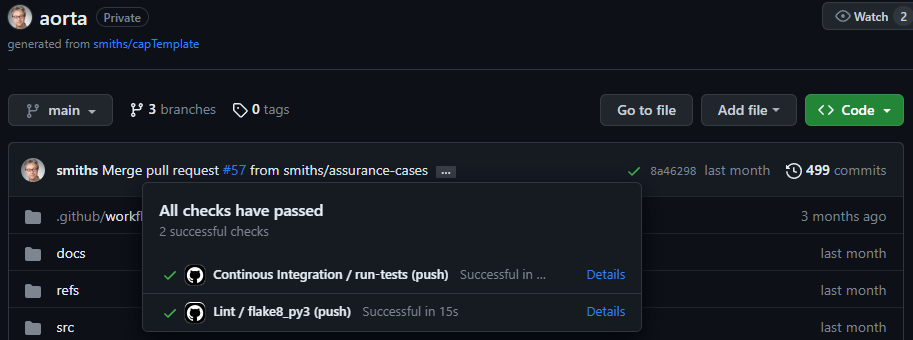
\includegraphics[width=0.9\textwidth]{figures/AC/GI/test_report.png}
    \caption[AGR Test Report]{AGR Test Report}
    \label{fig_agr_test_report}
\end{figure}

GitHub will email all the contributors when checks are not successful, so that the problem can be quickly addressed.

\section{The Design Documentation of the \progname{}}

This section discusses the design documents of \progname{}. There are multiple aspects of the design document to discuss:

\begin{enumerate}
\item System architecture, or high levels design.
\item Detailed design explaining how the algorithm works.
\end{enumerate}

The first item is presented with a Module Guide, and the second item is presented with a source code documentation generator, which generates the HTML documentation hosted on the web server.

\subsection{Module Guide}

An important document to show that the design is complete, correct, and consistent is the Module Guide (MG), which is attached as Appendix \ref{MG}. As explained previously, MG demonstrates the system architecture, or the high level design of the \progname{}. MG is a hierarchically-structured document, intended to allow both designers and maintainers to easily identify  the parts of the software that they must understand, without reading irrelevant details about other parts of the software \cite{ParnasEtAl1984}. 

The designer typically keeps these anticipated changes isolated to a single module so that if the change happens, only one module is impacted. The anticipated changes for AGR are listed in Figure~\ref{fig_agr_ac} below.

\begin{figure}[H]
    \centering
    \fbox{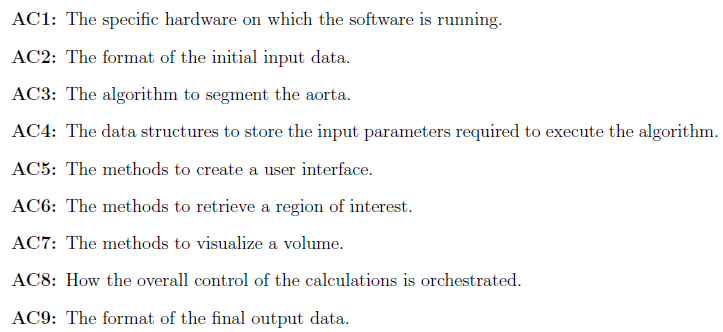
\includegraphics[width=\textwidth]{figures/AC/MG/Anticipated_Changes.png}}
    \caption[AGR Anticipated Changes]{AGR Anticipated Changes}
    \label{fig_agr_ac}
\end{figure}

Modules are decomposed according to the principle of “information hiding” proposed by Parnas et al. (1984) \citep{ParnasEtAl1984}. The secrets' field in a module decomposition is a brief statement of the design decision hidden by the module. The services' field specifies what the module will do without documenting how to do it. The module hierarchy and a part of the module decomposition is shown in Figure~\ref{fig_agr_modules} and Figure~\ref{fig_agr_md}. For each module, a suggestion for the implementing software is given under the ``Implemented By" title. If the entry is OS, this means that the module is provided by the operating system or by standard programming language libraries. AGR means the module will be implemented by the AGR software.

\begin{figure}[H]
    \centering
    \fbox{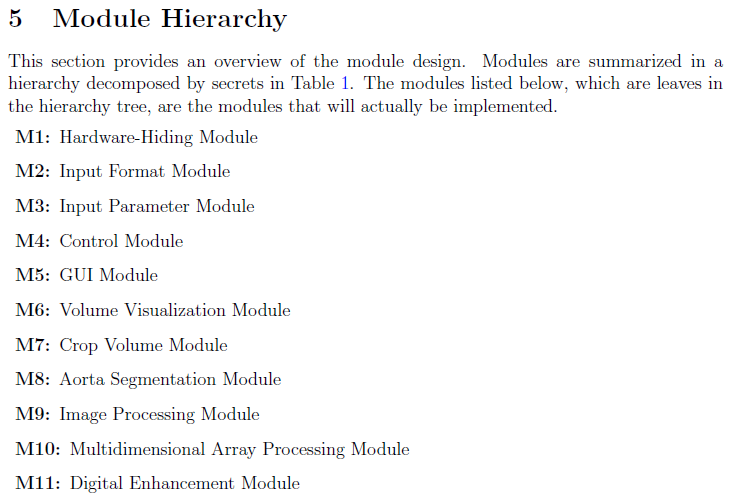
\includegraphics[width=\textwidth]{figures/AC/MG/Modules.png}}
    \caption[AGR Modules]{AGR Modules}
    \label{fig_agr_modules}
\end{figure}

\begin{figure}[H]
    \centering
    \fbox{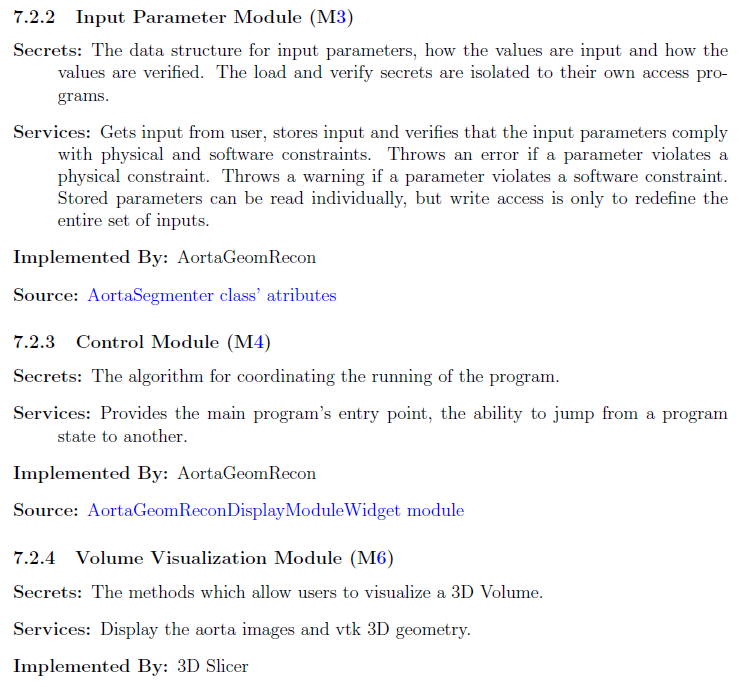
\includegraphics[width=\textwidth]{figures/AC/MG/Modules_Decomposition.png}}
    \caption[AGR Module Decomposition Example]{AGR Module Decomposition Example}
    \label{fig_agr_md}
\end{figure}

Traceability matrices show the relationships between the modules and the anticipated changes, and between the modules and the requirements, as shown in Figure~\ref{fig_agr_mtm}. The matrix shows all requirements are mapped to module, which is part of the evidence for E\_I.5\_3, under the GI.2 in Figure~\ref{fig_agr_ac_gi}.

\begin{figure}[H]
    \centering
    \fbox{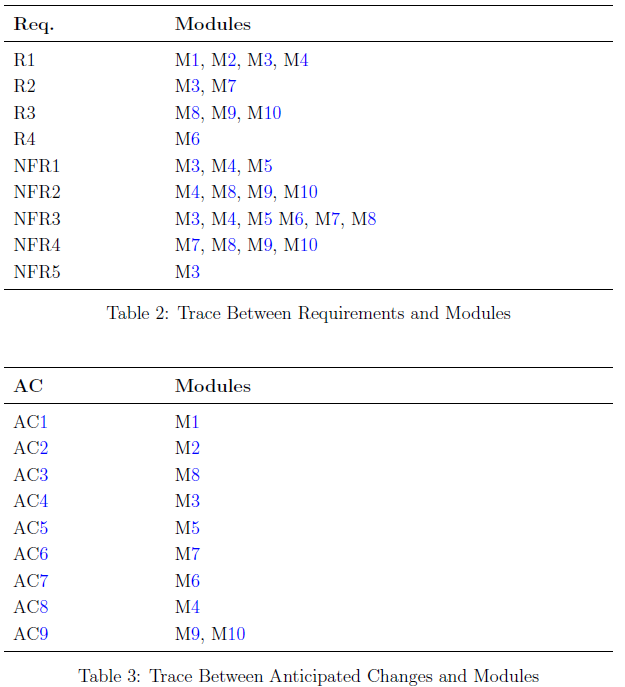
\includegraphics[width=0.7\textwidth]{figures/AC/MG/TM.png}}
    \caption[AGR Modules Traceability Matrices]{AGR Modules Traceability Matrices}
    \label{fig_agr_mtm}
\end{figure}

On top of relating the modules to the requirements, the actual source code is also mapped to the modules, which is strong evidence of our implementation complying with the requirements, as shown in Figure~\ref{fig_agr_mtm_modules_code}. Module 11, Digital Enhancement Module is an example of Module mapping to a piece of the source code. The comments on top indicate the source file where this piece of the source code is located, as well as the exact places within GitHub with the exact lines highlighted. This table demonstrates that the implemented modules all trace to the module guide modules, as stated in evidence E\_I.5\_0.

\begin{figure}[H]
    \centering
    \fbox{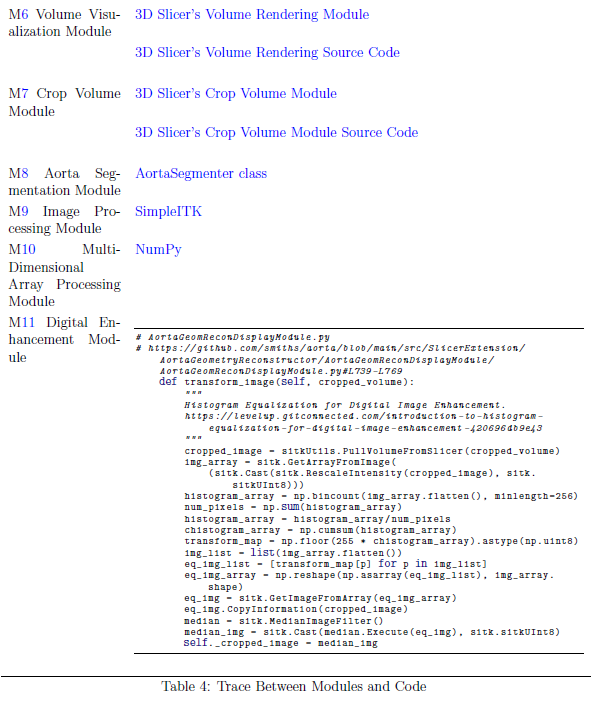
\includegraphics[width=0.9\textwidth]{figures/AC/MG/TM_modules_code.png}}
    \caption[AGR Part Of The Traceability Matrix On Modules And Code]{AGR Part Of The Traceability Matrix On Modules And Code}
    \label{fig_agr_mtm_modules_code}
\end{figure}

\subsection{Detailed Design Document}
The purpose of the Design Document \cite{DD} is to explain in detail how the algorithm works, and why it works. Similar to Section \ref{algo}, the design document explains in plain text the workflow of the algorithm. The design document is a piece of evidences that demonstrates unambiguity. Moreover, this document can let the domain expert do a design review  without reading the source codes directly,  which helps to build evidence E\_I.5\_2.

To show and automate the detailed design, we used Sphinx, a Python Documentation Generator that can build a module's documentation from the comments in the source code. Moreover, using reStructuredText to write the Algorithm Overview, we can build HTML code which can be published on a web server, as shown in Figure~\ref{fig_agr_dd}, which shows the index page of the \href{https://joviel25.github.io/AortaGR-design-document/index.html}{website}. 

\begin{figure}[H]
    \centering
    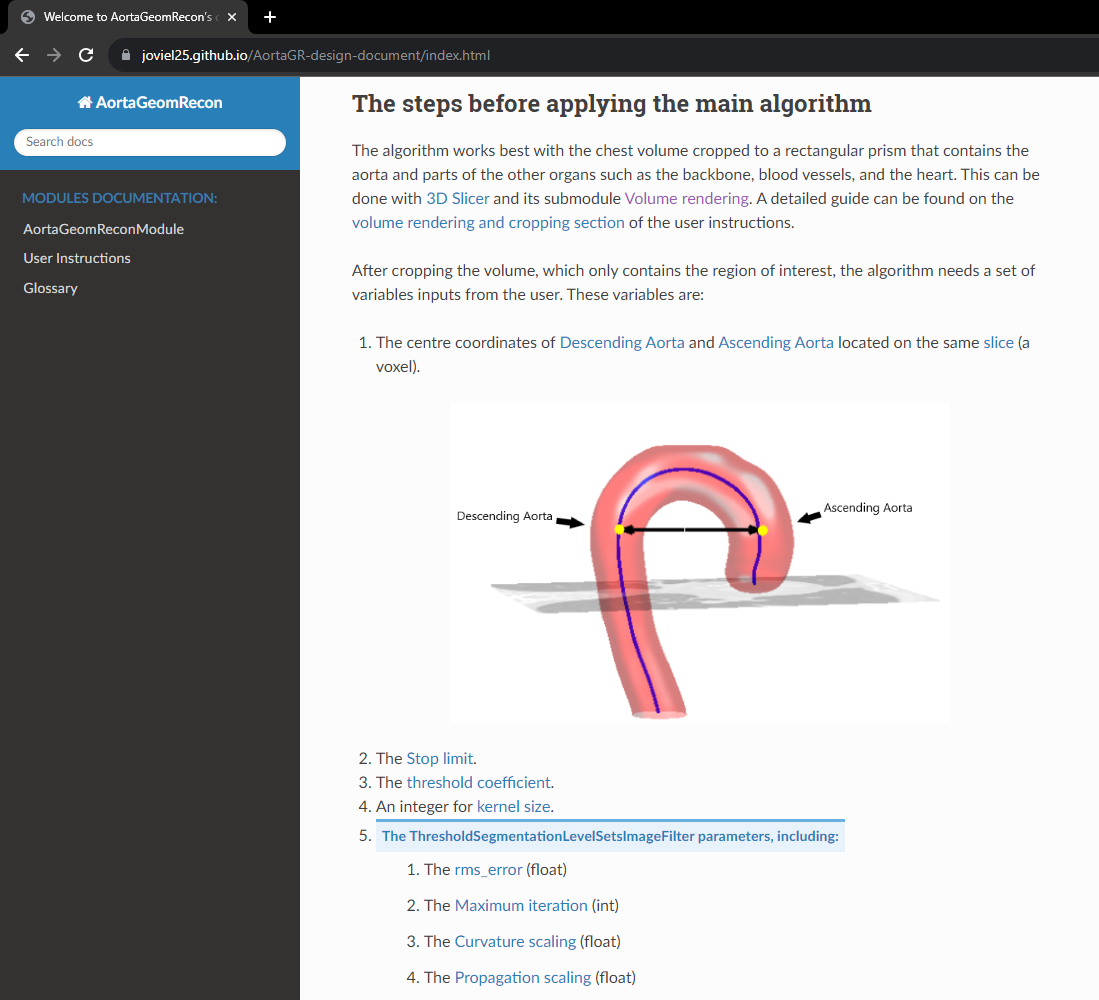
\includegraphics[width=0.65\textwidth]{figures/AC/DD/Main_page.png}
    \caption[AGR Design Document Website]{AGR Design Document Website}
    \label{fig_agr_dd}
\end{figure}

Another important section in the detailed design document is the Glossary. It provides a rich vocabulary of explanations, images, and links to the outside source to let the reader understands as much as possible. An excerpt from the Glossary is shown in Figure~\ref{fig_agr_dd_glossary}.

\begin{figure}[H]
    \centering
    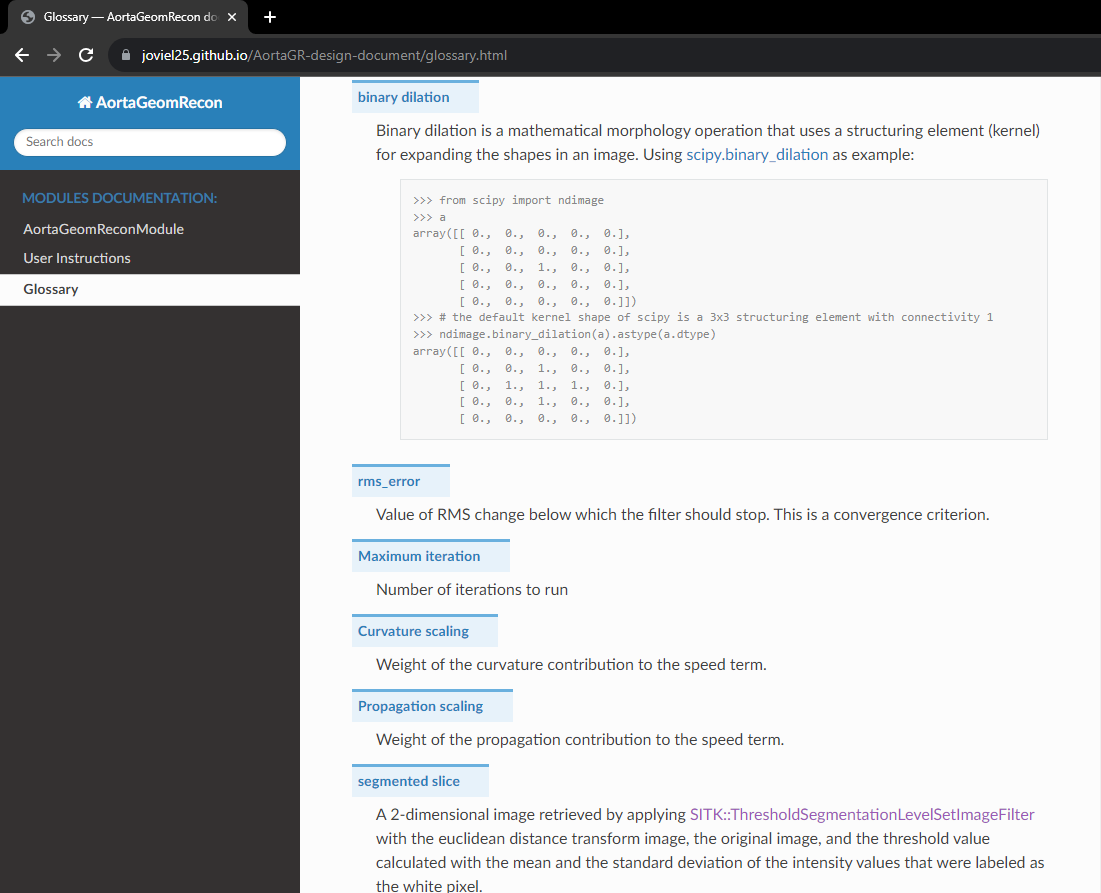
\includegraphics[width=\textwidth]{figures/AC/DD/Glossary.png}
    \caption[AGR Design Document Glossary]{AGR Design Document Glossary}
    \label{fig_agr_dd_glossary}
\end{figure}


\subsection{Algorithm Review}

The Algorithm Review started with a Code Walkthrough. A Code Walkthrough is a systematic and collaborative process in software development where a team of developers, designers, and stakeholders review and analyze a piece of code, typically with the aim of identifying defects, potential issues, and improvements \cite{Corporate_2023}. During a Code Walkthrough, participants examine the code line by line, discussing its design, functionality, readability, maintainability, and adherence to coding standards. The process involves both the author of the code and other team members, fostering knowledge sharing and collective learning. The goal is to catch issues and enhance the codebase through collective expertise.

We contrast a Code Review with an Algorithm Review. In an Algorithm Review, we present the algorithm to the domain expert and asking them if the detailed design fulfill the implementation objectives. In a Code Review, we are inspecting the implementation and verifying if the implementation has followed the design. 

In this section, we will discuss the Code Review with Kailin Chu, and the key takeaways from this meeting. Then, we will discuss the Algorithm Review with Dr. Dean Inglis, which was a meeting to reinforce our confidence in the design. Finally, we will briefly introduce the tools that we have used in both meetings.

\subsubsection{Code Review with Kailin Chu}
The Code Review was done with Kailin Chu, who is a biomedical engineering student at McMaster University. She produced the first version of the semi-automatic aorta segmentation algorithm as a summer researcher in 2021. The code review meeting took place on Thursday, April 20, 2023. The duration was about an hour. Along with Dr. Smith Spencer, we were aiming to increase our confidence in the code via a Code Walkthrough. The code walkthrough did not increase our confidence in the software because we quickly realized that an hour was not enough time to step through even a representative section of the code line by line. We quickly switched the purpose of the meeting to be a code review, so that we could understand the rationale behind Kailin's original code. This part of the meeting was only partially successful, because the code was developed by Kailin two years prior, so some details and design decisions had been forgotten. We also learned that some parameters were not set by theoretical considerations, but rather by trial and error. Despite that the meeting did not achieve its original goal, this meeting was still very helpful, because it enabled algorithm improvements. Learning that parts of the algorithm were based on trial-and-error freed me to consider changing it.

Originally, my method to generate a label image (Section \ref{label_map}) was not flexible to adjust its range based on the test case. This meant the segmentation on the aortic arch requires the algorithm to generate a label image to cover part of the descending aorta. However, this coverage is missing when executing on certain test cases, because the label image is generated using fixed index. The code review with Kailin provided the revelation that this part of her algorithm was partially based on trial and error. Learning that the original algorithm are partially arbitrary gave me the confidence to improve it using the idea of centroids. By using two centroids, one centroid on the ascending aorta and another on the descending aorta, the centroids can keep track of the most centered position of ascending aorta and descending aorta even when the aortic arch region is reached. Thus, it generates a better label image, and generates a more accurate segmentation result. Moreover, the execution time is reduced with the improved algorithm, because the improved algorithm only needs to perform one scan of the input volume. The original segmentation algorithm requires two scans of the input volume, each scan segments the descending and ascending aorta separately.

\subsubsection{Algorithm Review with Dr. Dean Inglis}

Since the experiment with Kailin Chu was only partially successful, we met with another reviewer. Rather than a code walkthrough or code review, we focused on the big picture of reviewing our algorithm. An algorithm review was conducted with Dr. Dean Inglis, an experienced professor, Medical Image Analyst, and Software Developer. This meeting happened on May 17, 2023, with a duration of about one and half hours. We presented our segmentation algorithm to him and requested validation of our approach, or suggestions for a potentially superior algorithm. Dr. Inglis provided his insights on the algorithm. These insights were meticulously recorded on the GitHub issue tracker. These insights will guide the developer responsible for enhancing the program.

This meeting significantly reinforced our confidence in both the software and our endeavors, because the methods discussed in the Section \ref{label_map}, \ref{distance_map}, and \ref{threshold} were very common in image analysis. We also learned that the level sets segmentation is also an often used technique for image segmentation. This indicates that the evidence E\_I.5 is accomplished.

\subsubsection{Tool used in Algorithm Review}

Spyder is a free and open source scientific environment written in Python, for Python, and designed by and for scientists, engineers and data analysts. The Variable Explorer shown in Figure\ref{fig_spyder_ve} allows the user to interactively browse the variables and the objects in debugging mode \cite{raybaut2009spyder}.

\begin{figure}[H]
    \centering
    \fbox{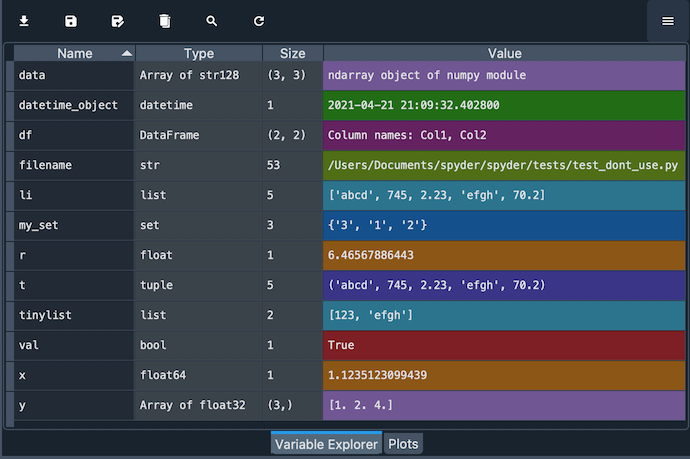
\includegraphics[width=0.8\textwidth]{figures/AC/AR/variable-explorer-standard.png}}
    \caption[Spyder Variable Explorer]{Spyder Variable Explorer \cite{raybaut2009spyder}}
    \label{fig_spyder_ve}
\end{figure}

This feature allows us to execute the program step by step, and see what happens to the variable (segmentation result) when executing the segmentation algorithm. This was very valuable for our code walkthrough/review meeting.

\section{Assurance Case for Operational Assumptions}

\begin{figure}[H]
    \centering
    \fbox{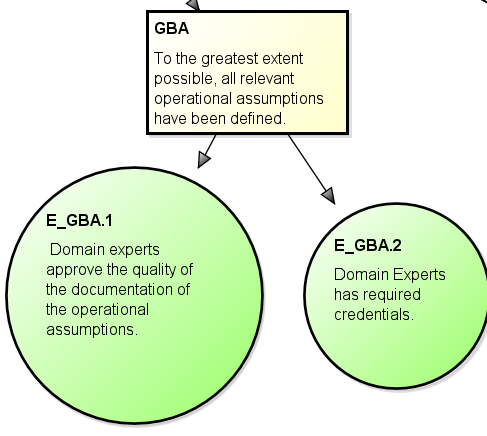
\includegraphics[width=0.5\textwidth]{figures/AC/GBA/GBA.png}}
    \caption[AGR Assurance Case Operational Assumptions]{AGR Assurance Case Operational Assumptions}
    \label{fig_agr_ac_gba}
\end{figure}

The evidence for the statement ``To the greatest extent possible, all relevant operational assumptions have been defined" is quite simple as all that is required is a qualified Domain expert to approve the quality of the documentation. However, finalizing this evidence takes significant effort from the beginning of the project to the end of the project, because of the need to continuously improve the quality of the content matching the most recent updates of the software.

In this section, we will present two methods to define all relevant operational assumptions. The first method is a User Manual, which is written in plain text and multiple screenshots. The second method is a User Instructional Video, which includes voice over to guide the user step by step.

\subsection{User Manual}\label{user_manual}
A user manual serves the purpose of documenting all operational assumptions. When the user gets unexpected results by using this software, they should be able to refer to the user manual to see what pieces are different. Our user manual is initially located in GitHub repo's README, as shown in Figure~\ref{fig_agr_git_um}, which is only available to the developers invited as the GitHub project contributors. The content includes the installation of the software, importing the extension modules, import inputs data, and perform segmentation. The user manual is also available publicly on the \href{https://joviel25.github.io/AortaGR-design-document/UserInstructions.html}{design document website}, for users that are not the repository contributors.

\begin{figure}[H]
    \centering
    \fbox{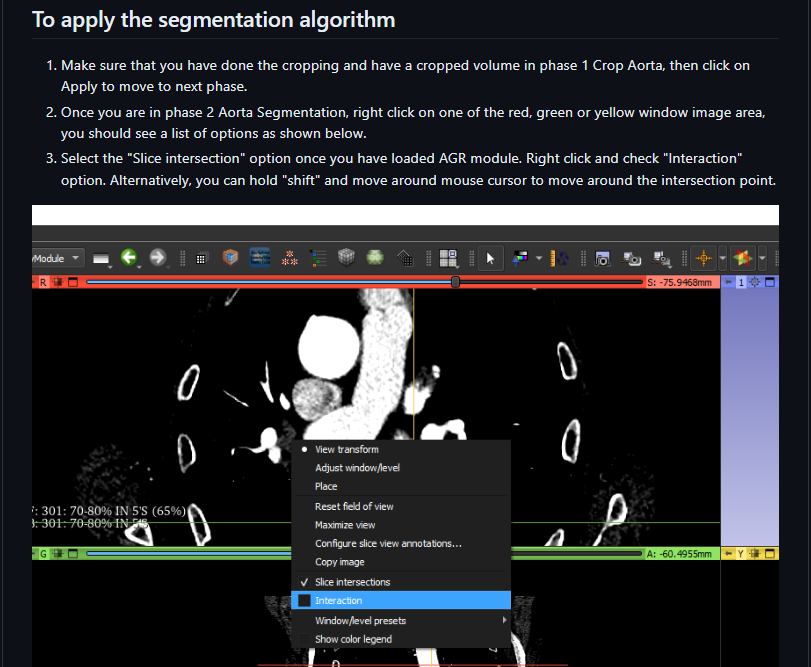
\includegraphics[width=0.9\textwidth]{figures/AC/GBA/User_manual.png}}
    \caption[AGR User Manual On GitHub README]{AGR User Manual On GitHub README}
    \label{fig_agr_git_um}
\end{figure}


\subsection{User Instruction Video}\label{user_instruction_video}
Videos are an effective way to engage your audience and deliver information in a way that's easy to follow along and understand. A better instructional content is a YouTube Video where we make step-by-step instruction with voice over to instruct the user. Figure~\ref{fig_video} shows a snapshot  of video on YouTube. The video is not listed publicly on YouTube, but the users who have access to the GitHub repository or Design Document website can access this video by the \href{https://www.youtube.com/watch?v=1eK5k6bazNs}{URL link}.

\begin{figure}[H]
    \centering
    \fbox{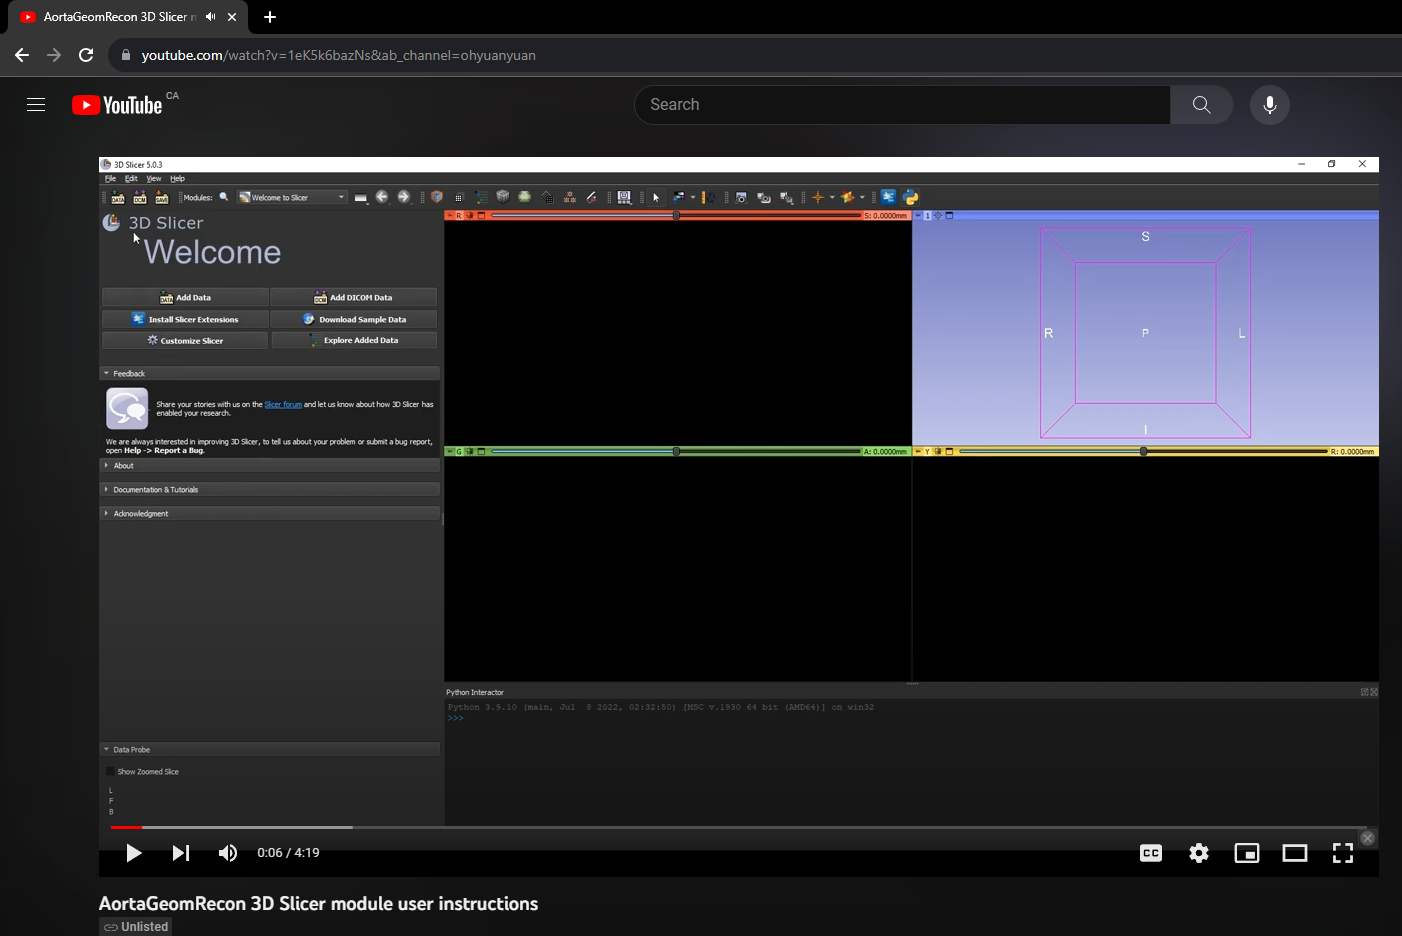
\includegraphics[width=0.8\textwidth]{figures/AC/GBA/User_instructions_video.png}}
    \caption[AGR User Instructions on YouTube]{AGR User Instructions on YouTube}
    \label{fig_video}
\end{figure}


\section{Assurance Case for Inputs Assumptions}

\begin{figure}[H]
    \centering
    \fbox{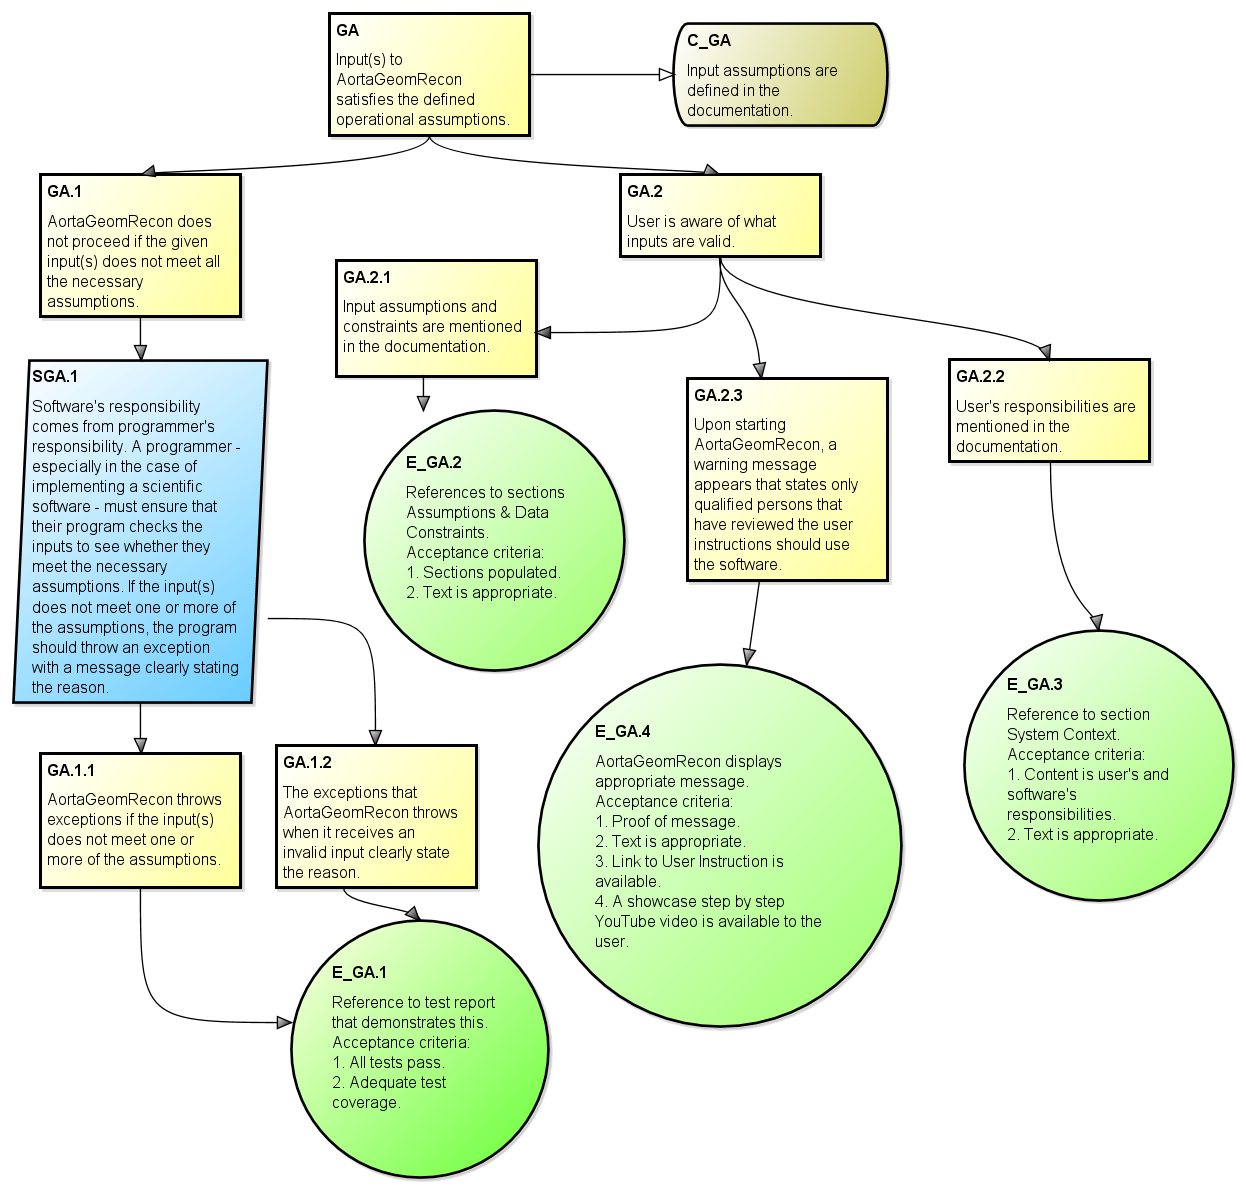
\includegraphics[width=\textwidth]{figures/AC/GA/GSN_GA.png}}
    \caption[AGR Assurance Case Inputs Assumptions]{AGR Assurance Case Inputs Assumptions}
    \label{fig_agr_ac_ga}
\end{figure}

Figure~\ref{fig_agr_ac_ga} shows our last assurance case, GA. This statement requires the user know what inputs are valid, and only uses the valid inputs in the software. The user documentation described in sections \ref{user_manual} and \ref{user_instruction_video} communicate this information to the user. When the software gets unexpected inputs, it should not proceed to the next step, which could result in unexpected results.

\subsection{AortaGoemRecon's Control Sequence}

In the logic of the control sequence implemented as the 3D Slicer scripted module, the appropriate inputs must meet the necessary assumptions before proceeding to the next step.
In phase one, a cropped volume with a name that includes the string ``cropped" must be present in the node storage, where a cropped volume created by Crop Volume module is automatically named with the string ``cropped" as part of the volume's name. Otherwise, the user cannot go to the next phase through normal operation. In phase two, the aorta seeds must be provided to continue to the segmentation. Although it does not directly provide evidence, it will help passing the test mentioned in the test report, as discussed in E\_GA.1 in Figure~\ref{fig_agr_ac_ga}.

\subsection{AortaGoemRecon's Graphical User Interface}

AortaGeomRecon's Graphical User Interface, discussed in Section \ref{GUI}, reduces the problems with user input by limiting the user's ability to enter any value possible. The hyperparameters shown in Figure~\ref{fig_module_ui} have a minimum and maximum value limitation. This is an improvement to the prior Jupyter Notebook where the users have as much freedom as they want to modify any hard-coded parameter in the code. Similarly, the implementation of GUI does not provide evidence, but it will help to build the evidence for E\_GA.1 discussed in Figure~\ref{fig_agr_ac_ga}.

\subsection{Warning Message}

As we initially planned, the references to sections Assumptions, Data Constraints, and System Context is available in the User Manual and User Instruction Video, where we showed the user how to import DICOM patient's data, and operate on the inputs' data to get a segmentation result. This implies that the requirements of  the evidences E\_GA.2, E\_GA.3 and E\_GA.4 are met. A user who has read the User Manual and watched the instruction video should know what inputs are valid. Therefore, in the AGR module, we need to effectively guide the user to the User Manual, whether the user has used this software before or is a first time user.

\begin{figure}[H]
    \centering
    \fbox{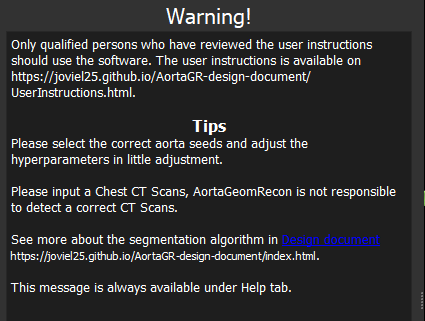
\includegraphics[width=0.6\textwidth]{figures/AC/GA/AGR_warning.png}}
    \caption[AGR Warning Message]{AGR Warning Message}
    \label{fig_agr_ac_wm}
\end{figure}

As mentioned in Section \ref{module_workflow}, when the user first starts 3D Slicer and click on the AGR module, the warning message in Figure \ref{fig_agr_ac_wm} appears. This is  the appropriate message as stated in E\_GA.4. The user must clicks on the Confirm button to continue to the next steps. With the warning message shown to the user, it is now the user's responsibility to use the valid inputs for AGR, so that the program will deliver the correct outputs if the other operations are performed correctly. 